
% WARNING!  Do not type any of the following 10 characters except as directed:
%                &   $   #   %   _   {   }   ^   ~   \   
%
%%
%%  default option for pdfx.sty  if not specified on the command-line.
\providecommand{\pdfxopt}{a-1b}
%% 
%%  Use  {filecontents}  for the  .xmpdata file before input encoding is specified.
%%
%%%%%%%%%%%%%%%%%%%%%%%%%%%%%%%%%%%%%%%%%%%%%%%%%%%
\begin{filecontents*}{\jobname.xmpdata}
	% a macro definition, used below
	\pdfxEnableCommands{% simple macro definitions can be provided everything expands to characters
	 \def\RossPete{Ross \& Pete}
	 }
	\Title{MAT335 Notes}%  *not* set by LaTeX's  \title
	\Author{Jason Siefken\sep et al.}% *not* set by LaTeX's \author
	\Subject{Chaos, Fractals, Dynamics notes/exercises}
	\Keywords{dynamics\sep fractals\sep chaos\sep mathematics\sep notes} 
	\Org{University of Toronto}
	\CreatorTool{LaTeX + pdfx.sty with options \pdfxopt}
	\Copyright{Jason Siefken}
	\WebStatement{https://github.com/siefkenj/IBLLinearAlgebra/}% should be URL to copyright statement on the web
	\CoverDisplayDate{2019}
	\CoverDate{2019-08-014}%  must be in format  YYYY-MM-DD  or  YYYY-MM
	\Doi{0.0.0.0}%
	%
	% setting the color profile, these reproduce the defaults; use your own, if required 
	%
	% RGB is used with PDF/A (4 parameters):
	\setRGBcolorprofile{sRGB_IEC61966-2-1_black_scaled.icc}{sRGB_IEC61966-2-1_black_scaled}{sRGB IEC61966 v2.1 with black scaling}{http://www.color.org}
	%
	%  For Adobe Color Profiles, set the directory for your system
	%
	%  e.g.  on Mac OS X
	%  What is it under Windows ?
	%
	\gdef\ColorProfileDir{/Library/Application Support/Adobe/Color/Profiles/Recommended/}
	% 
	%  For available profiles, see file  AdobeColorProfiles.tex
	%  For PDF/X-4p or PDF/X-5pg   see file  AdobeExternalProfiles.tex  
	%
	%  Now you can use the macros defined in those files:
	 \FOGRAXXXIX 
	%
	% or CMYK is used with  PDF/X (4 parameters)
	% \setCMYKcolorprofile{\ColorProfileDir coated_FOGRA39L_argl.icc}{Coated FOGRA39}{FOGRA39 (ISO Coated v2 300\%\space (ECI))}{http://www.color.org}
\end{filecontents*}

\documentclass{problemset}


% pdfx will set color profile etc. information appropriately, so the pdf renders
% consistently across devices. But, it doesn't work with the xelatex-based tectonics
\usepackage{ifxetex}
	\usepackage[utf8]{inputenc}
\ifxetex
\else
	\usepackage[a-3u]{pdfx}
	\hypersetup{hidelinks=true, linkcolor = {0 0 1} }
\fi

%%%
% import all needed packages and macros
%%%
\usepackage[yyyymmdd]{datetime}
%%
%% All packages and macros needed for the problemsets
%%

\usepackage{amsmath}

\usepackage{lipsum}
%\usepackage{showframe}
%\usepackage{layout}


\usepackage[charter,cal=cmcal]{mathdesign} %different font
%\usepackage{avant}

\usepackage{microtype}
\usepackage{mathtools}
\usepackage{etoolbox}
%\usepackage{amsfonts}
%\usepackage{amssymb}
\usepackage{graphicx}
\usepackage[inline]{enumitem}
\usepackage{xparse}
\usepackage{ifthen}
\usepackage{graphicx}
\usepackage{caption}
\usepackage{subcaption}
\usepackage{color}
\usepackage{tikz}
	\usetikzlibrary{fit}
	\usetikzlibrary{fadings}
	\usetikzlibrary{calc}
	\tikzset{>=latex}
	\usetikzlibrary{cd}
	\usetikzlibrary{spy}
\usepackage{fancyhdr}
\usepackage{calc}
\usepackage{wrapfig}
\usepackage{marginnote}
\usepackage{mparhack}
\usepackage{marginfix}
\usepackage{pdfpages}

%\usepackage[
%  linktocpage=false,      % no page numbers are clickable
%  colorlinks=false,       % no color
%  breaklinks=true,        % break URLs
%  bookmarks,              % creates bookmarks in pdf
%  hyperfootnotes=true,    % clickable footnotes
%  pdfborder={0 0 0},      % for removing borders around links
%  bookmarksnumbered=true, % If Acrobat bookmarks are requested, include section numbers.
%  bookmarksopen=false,    % If Acrobat bookmarks are requested, show them with all the subtrees expanded.
%  %hidelinks=true,
%  %linkcolor=blue,
%  %citecolor=blue,
%  %urlcolor=blue,
%  pdfpagemode={UseOutlines}, % show pdf bookmarks (indices) on startup; does not function all the time
%  pdftitle={...}, % title
%  pdfauthor={...}, % author
%  pdfkeywords={...}, % subject of the document
%  pdfsubject={...}, % list of keywords
%  pdfmenubar=true,        % make PDF viewer’s menu bar visible
%  pdfpagelabels,
%]{hyperref}
%\usepackage[hidelinks,]{hyperref}
\usepackage{fnpct} % fancy footnote spacing
\usepackage{bm}
\usepackage{systeme}
\usepackage{datatool}% http://ctan.org/pkg/datatool for sorted lists
\usepackage{xspace}



\usepackage{pgfplots}
\pgfplotsset{compat=newest}
	\usepgfplotslibrary{fillbetween}
%%%
% Useful Linear Algebra macros
%%%
\newcommand{\declarecommand}[1]{\providecommand{#1}{}\renewcommand{#1}}
\declarecommand{\R}{\mathbb{R}}  % we don't care if it's already defined.  We really want *this* command!
\declarecommand{\Z}{\mathbb{Z}}
\declarecommand{\Q}{\mathbb{Q}}
\declarecommand{\N}{\mathbb{N}}
\declarecommand{\C}{\mathbb{C}}
\declarecommand{\d}{\mathrm{d}}
\declarecommand{\dd}{\mathbbm{d}} % exterior derivative
\DeclareMathOperator{\Span}{span}
\DeclareMathOperator{\Img}{img}
\DeclareMathOperator{\Id}{id}
\DeclareMathOperator{\Ident}{\Id}
\DeclareMathOperator{\Vol}{Vol}
\DeclareMathOperator{\VolChange}{Vol\hspace{1.5pt}Change}
\DeclareMathOperator{\Range}{range}
\DeclareMathOperator{\Rref}{rref}
\DeclareMathOperator{\Rank}{rank}
\DeclareMathOperator{\Comp}{\Vcomp}
\DeclareMathOperator{\Vcomp}{v\hspace{1pt}comp}
\DeclareMathOperator{\Null}{null}
\DeclareMathOperator{\Nullity}{nullity}
\DeclareMathOperator{\Char}{char}
\DeclareMathOperator{\Proj}{proj}
\DeclareMathOperator{\Flux}{Flux}
\DeclareMathOperator{\Circ}{Circ}
\DeclareMathOperator{\chr}{char}
\DeclareMathOperator{\Dim}{dim}
\DeclareMathOperator{\Perp}{perp}
\DeclareMathOperator{\Ker}{kernel}
\DeclareMathOperator{\Row}{row}
\DeclareMathOperator{\Col}{col}
\DeclareMathOperator{\Rep}{Rep}
\newcommand{\BasisChange}[2]{[#2\!\leftarrow\!#1]}
\newcommand{\proj}{\Proj}
\newcommand{\rref}{\Rref}
\newcommand{\xhat}{{\vec e_1}}
\newcommand{\yhat}{{\vec e_2}}
\newcommand{\zhat}{{\vec e_3}}
\newcommand{\sbasis}[1]{\vec { e}_{#1}}
\newcommand{\mat}[1]{\begin{bmatrix*}[r]#1\end{bmatrix*}}
\newcommand{\matc}[1]{\begin{bmatrix}#1\end{bmatrix}}
\newcommand{\formarg}[2]{\big(#1;\, #2\big)}
\DeclarePairedDelimiter\abs{\lvert}{\rvert}
\DeclarePairedDelimiter\Abs{\lvert}{\rvert}
\DeclarePairedDelimiter\norm{\lVert}{\rVert}
\newcommand{\Norm}[1]{\norm{#1}}
% just to make sure it exists
\providecommand\given{}
% can be useful to refer to this outside \Set
\newcommand\SetSymbol[1][]{%
	\nonscript\::%
	\allowbreak
	\nonscript\:
	\mathopen{}}
\DeclarePairedDelimiterX\Set[1]\{\}{%
	\renewcommand\given{\SetSymbol[\delimsize]}
	#1
}

\newcommand{\scaledgrid}[1]{%
	\begin{tikzpicture}[scale=#1]
		\draw[thin, white!20!black, dotted] (-4.1,-4.1) grid (4.1,4.1);
		\draw[ <->] (-4.3,0) -- (4.3,0);
		\draw[ <->] (0,-4.3) -- (0,4.3);
	\end{tikzpicture}
}
\newcommand{\scaledshortgrid}[1]{%
	\begin{tikzpicture}[scale=#1]
		\draw[thin, white!20!black, dotted] (-4.1,-2.1) grid (4.1,2.1);
		\draw[ <->] (-4.3,0) -- (4.3,0);
		\draw[ <->] (0,-2.3) -- (0,2.3);
	\end{tikzpicture}
}
\newcommand{\singlegrid}{\scaledgrid{1}}
\newcommand{\doublegrid}{\mbox{\scaledgrid{.9}\scaledgrid{.9}}\par}
\newcommand{\triplegrid}{\mbox{\scaledgrid{.6}\scaledgrid{.6}\scaledgrid{.6}}\par}

% labels for source attributions
\NewDocumentCommand{\beezer}{o}{%
	\IfNoValueTF{#1}{%
		{\color{blue}\sffamily{B}}%
	}{%
		{\color{blue}\sffamily{B}}%  XXX Todo, make this href to the appropriate problem number
	}\xspace%
}
\NewDocumentCommand{\hefferon}{o}{%
	\IfNoValueTF{#1}{%
		{\color{blue}\sffamily{H}}%
	}{%
		{\color{blue}\sffamily{H}}%  XXX Todo, make this href to the appropriate problem number
	}\xspace%
}


% in non-xelatex engines, hyperref is loaded by `pdfx`. If `pdfx` is not loaded, load it here.
\ifxetex
	\usepackage{hyperref}
	\hypersetup{hidelinks=true, linkcolor = {0 0 1} }
\else
\fi

%%%
% Set up the footers to have the correct copyright notices
%%%

\fancypagestyle{siefken}{%
	\rfoot{\footnotesize\it \copyright\,Jason Siefken, 2015--2019 \ \makebox(30,5){
\includegraphics[height=1.2em]{by-sa.pdf}}}
	\lfoot{}
	\renewcommand{\headrulewidth}{0pt}
}
\fancypagestyle{iola}{%
	\rfoot{\footnotesize\it \copyright\,IOLA Team \url{iola.math.vt.edu} \ \makebox(30,5){\includegraphics[height=2.2em]{images/iolalogo.png}}}
	\lfoot{}
	\renewcommand{\headrulewidth}{0pt}
}

\DeclareDocumentEnvironment{iola}{o}{%
	\newpage
	\pagestyle{iola}
}{%
	\newpage
}


%%
% Allow hiding of environments
%%
\usepackage{environ}% http://ctan.org/pkg/environ
\makeatletter
\newcommand{\voidenvironment}[1]{%
  \expandafter\providecommand\csname env@#1@save@env\endcsname{}%
  \expandafter\providecommand\csname env@#1@process\endcsname{}%
  \@ifundefined{#1}{}{\RenewEnviron{#1}{}}%
}
\makeatother
% allow pagebreaks that only display in `standard` mode
\newcommand{\displayonlynewpage}{\begin{displayonly}\newpage\end{displayonly}}
% allow pagebreaks that only display in `book` mode
\newcommand{\bookonlynewpage}{\begin{bookonly}\newpage\end{bookonly}}

%
% Set up the three render modes: standard, instructor, and solutions.
% These render with varying amounts of extra data (like solutions and notes)
%
\newtoggle{instructor}
\newtoggle{standard}
\newtoggle{solutions}
\newtoggle{book}
\newcommand{\setinstructor}{
	\toggletrue{instructor}
	\togglefalse{standard}
	\togglefalse{solutions}
	\togglefalse{book}
}
\newcommand{\setstandard}{
	\togglefalse{instructor}
	\toggletrue{standard}
	\togglefalse{solutions}
	\togglefalse{book}
}
\newcommand{\setsolutions}{
	\togglefalse{instructor}
	\togglefalse{standard}
	\toggletrue{solutions}
	\togglefalse{book}
}
\newcommand{\setbook}{
	\togglefalse{instructor}
	\togglefalse{standard}
	\togglefalse{solutions}
	\toggletrue{book}
	\setbookgeometry
}

%
% Infer the document level from the \jobname
%
\usepackage{xstring}
\IfSubStr{\jobname}{\detokenize{book}}{\setbook}{
	\IfSubStr{\jobname}{\detokenize{solutions}}{\setsolutions}{
		\IfSubStr{\jobname}{\detokenize{instructor}}{\setinstructor}{
			\setstandard
		}
	}
}

%
% Hide the non-problem environments
%
\newcommand{\coversubtitle}{} % we override the subtitle in each mode, so make sure the command exists to override.
\iftoggle{instructor}{
	\voidenvironment{module}
	\voidenvironment{bookonly}
	\voidenvironment{displayonly}
	\renewcommand{\coversubtitle}{Instructor Guide}
}{}
\iftoggle{solutions}{
	\voidenvironment{module}
	\voidenvironment{bookonly}
	\voidenvironment{displayonly}
	\voidenvironment{lesson}
	\voidenvironment{notes}
	\renewcommand{\coversubtitle}{Solutions}
}{}
\iftoggle{standard}{
	\voidenvironment{module}
	\voidenvironment{bookonly}
	\voidenvironment{solution}
	\voidenvironment{annotation}
	\voidenvironment{lesson}
	\renewcommand{\coversubtitle}{MAT335 Notes}
}{}
\iftoggle{book}{
	\voidenvironment{displayonly}
	\voidenvironment{solution}
	\voidenvironment{annotation}
	\voidenvironment{lesson}
	\renewcommand{\coversubtitle}{{\hspace{-5pt}\begin{tabular}{l}MAT223 Workbook\\\small\today{} Edition\end{tabular}}}
}{}
%\voidenvironment{solution}
%\voidenvironment{annotation}
%\voidenvironment{lesson}
%%\voidenvironment{notes}
%%\voidenvironment{displayonly}

\renewcommand{\P}{\mathbb{P}}
\renewcommand{\C}{\mathbb{C}}
\newcommand{\E}{\mathbb{E}}


\begin{document}

%%
%% End Definitions
%%






\pagestyle{empty}

\begin{tikzpicture}[remember picture,overlay]
    \coordinate (A) at (current page.north west);
    \coordinate (B) at (current page.south east);
    \draw[red, very thick]%, cap=round]
    (A) -- (B);
    \node[anchor=north west, inner sep=0cm] at (A) {\includegraphics[width=\pagewidth]{images/cover-Nayan-Saxena.pdf}};
    \node[anchor=north east, white] at (current page.north east) {Cover by Nayan Saxena}; 
\end{tikzpicture}
%\includepdf[noautoscale=true, width=\paperwidth]{images/cover-Nayan-Saxena.pdf}

%\begin{tikzpicture}[remember picture,overlay, shift={(current page.north west)}, >=latex]
%	\definecolor{coverblue}{HTML}{ffd33c}
%	\definecolor{coverpink}{HTML}{ff97e8}
%	\definecolor{coveraccentpink}{HTML}{ffd33c}
%	\definecolor{coverorange}{HTML}{ffffff}
%	\definecolor{covershade}{HTML}{3f004d}
%
%	\fill[black] (0,0) rectangle (\pagewidth,\pageheight) node {Hi there};
%	\draw[black] (0,0) -- (-10,-10) node {Hi the};
%
%
%%	\begin{scope}
%%	%	\node[anchor=south east,inner sep=0pt,outer sep=0pt,] 
%%	%	at (current page.south east) {\includegraphics[width=\paperwidth, height=\paperheight]{images/orangeback.jpg}};
%%
%%		\fill[path fading=north,covershade] (0,2.2in) rectangle ([yshift=-1.01in, xshift=2pt]current page.north east);
%%		\fill[covershade] (0,-1in) rectangle ([yshift=-2.05in]current page.north east);
%%		\fill[path fading=south, covershade] (0,-2in) rectangle ([xshift=1in,yshift=2in]current page.south east);
%%	\end{scope}
%%
%%
%%  \begin{scope}[yscale=-1, xscale=1, x=2.7pt, y=2.7pt,line join=miter,line cap=butt,line width=1.3pt, yshift=2.3cm, xshift=.7cm,
%%	  ]
%%
%%	  \coordinate (E) at (57.55,23.15);
%%	  \coordinate (A) at (195.3,27.9);
%%	  \coordinate (C) at (195.3,104);
%%	  \coordinate (SUB) at (141, 30);
%%		
%%  \end{scope}
%%
%%  	\coordinate (X) at (3, -15);
%%	\path (E) --  (C)  
%%		coordinate[pos=0] (X1)
%%		coordinate[pos=.017] (X2)
%%		coordinate[pos=.08] (X3)
%%		coordinate[pos=.2] (X4)
%%		coordinate[pos=.5] (X5)
%%		coordinate[pos=1] (X6)
%%		-- (A);
%%	\draw[coverpink, line width=1.3pt] (E) --  (C)  
%%		-- (A);
%%	\begin{scope}[coverorange, line width=0.5pt]
%%		\draw[->] 
%%			(X) -- (X1) node[pos=.5, above left] {\Large $\vec u$};
%%		\draw[->] 
%%			(X) -- (X2);
%%		\draw[->] 
%%			(X) -- (X3);
%%		\draw[->] 
%%			(X) -- (X4);
%%		\draw[->, coveraccentpink, line width=1.3pt] 
%%			(X) -- (X5) node[pos=.6, below right] {\Large $\vec w_{\alpha}=\alpha {\color{coverorange}\vec u} + (1-\alpha){\color{coverorange}\vec v}$};
%%		\draw[->] 
%%			(X) -- (X6) node[pos=.7, below right] {\Large $\vec v$};
%%	\end{scope}
%%
%%	\path[white] (SUB) node[anchor=north west] {\Large \bfseries \sffamily \coversubtitle};
%%
%%\newcommand{\authornames}{\huge \sffamily \bfseries \begin{tabular}{r}Jason Siefken\end{tabular}}
%%	\newcommand{\ypadd}{.5em}
%%	\newcommand{\xpadd}{1em}
%%
%%	\draw (0, -24) node[right, xshift=10em] (AUTHOR) {\phantom{\authornames}};
%%	\path let \p1 = (AUTHOR.north) in coordinate (Ab1) at (0,\y1+\ypadd);
%%	\path let \p1 = (AUTHOR.north east) in coordinate (Ab2) at (\x1+\xpadd,\y1+\ypadd);
%%	\path let \p1 = (AUTHOR.south east) in coordinate (Ab3) at (\x1+\xpadd,\y1-\ypadd);
%%	\path let \p1 = (AUTHOR.south) in coordinate (Ab4) at (0,\y1-\ypadd);
%%
%%	\path[fill=covershade, path fading=west, opacity=.8] (Ab1) -- (Ab2) -- (Ab3) -- (Ab4);
%%	\draw[covershade!80!black, line width=1.3pt] (Ab1) -- (Ab2) -- (Ab3) -- (Ab4);
%%	\draw (0, -24) node[right, xshift=10em, white] (AUTHOR) {\authornames};
%
%\end{tikzpicture}


\newpage


\newcommand{\standardintro}{
\begin{center}
{\huge\bf Inquiry Based Linear Algebra}\\

\vspace{.7in}
{
\it \copyright\,Jason Siefken, 2016--2019 \\
Creative Commons By-Attribution Share-Alike\, \makebox(30,5){
\includegraphics[height=1.2em]{by-sa.pdf}}
}
\end{center}

\section*{About the Document}

This document is a hybrid of many linear algebra resources, including those of
the IOLA (Inquiry Oriented Linear Algebra) project and Jason Siefken's
IBL Linear Algebra project.

This document is a mix of short problems and more involved exploratory question. A typical
class day looks like:
\begin{enumerate}
	\item {\bf Introduction by instructor.} This may involve giving a definition,
		a broader context for the day's topics, or answering questions.

	\item {\bf Students work on problems.} Students work individually or in pairs/small groups
		on the prescribed problem. During this time the instructor moves
		around the room addressing questions that students may have and giving
		one-on-one coaching.

	\item {\bf Instructor intervention.} When most students have successfully solved
		the problem, the instructor refocuses the class by providing an
		explanation or soliciting explanations from students.
		This is also time for the instructor to ensure that everyone has
		understood the main point of the exercise (since it is sometimes
		easy to miss the point!).

		If students are having trouble, the instructor can give hints
		and additional guidance to ensure students' struggle is productive.

	\item {\bf Repeat step 2.}
\end{enumerate}

Using this format, students are thinking (and happily so) most of the class. Further,
after struggling with a question, students are especially primed to hear the insights of the instructor.

These problems are geared towards concepts instead of computation, though some problems
focus on simple computation. The questions also have a geometric lean. Vectors are initially
introduced with familiar coordinate notation, but eventually, coordinates are understood to be
\emph{representations} of vectors rather than ``true'' geometric vectors, and objects like the
determinant are defined via oriented volumes rather than formulas involving matrix entries.

\bigskip
{\bf License} Unless otherwise mentioned, pages of this document are licensed under
the Creative Commons By-Attribution Share-Alike License. That means, you are free
to use, copy, and modify this document provided that you provide attribution to the
previous copyright holders and you release your derivative work under the same license.
Full text of the license is at \url{http://creativecommons.org/licenses/by-sa/4.0/}

If you modify this document, you may add your name to the copyright list. Also,
if you think your contributions would be helpful to others, consider making a
pull request, or opening an \emph{issue} at \url{https://github.com/siefkenj/IBLLinearAlgebra}

Content from other sources is reproduced here with permission and retains the
Author's copyright. Please see the footnote of each page to verify the
copyright.

\newpage
}


\setcounter{page}{1}
\pagestyle{siefken}


\addcontentsline{toc}{chapter}{Lessons}

	\section*{Dynamical Systems}

	\begin{definition}[Dynamical System]
		A pair $(T,X)$ is called a \emph{dynamical system} if
		$X$ is a set and $T:X\to X$ is a function. In the context of
		a dynamical system, $T$ is often called a \emph{transformation}.
	\end{definition}

	This definition is very general, and most things you encounter could be considered
	a dynamical system. For example, if $X=\{\text{air molecules and their positions on earth}\}$
	and $T:X\to X$ is the result of the wind blowing for one second, then $(T,X)$ is a dynamical system.
	Alternatively, we could take the state of your computer's memory (RAM) to be a set and your processor executing a single
	instruction to be a transformation.

	It's hard to say much about general dynamical systems.
	However, throughout the course, we will find ways to classify dynamical systems. Once we ``narrow the field'',
	we'll be able to say lot's of interesting things.

	\subsection*{Newton's Method}
	Newton's method is a way of using tangent-line approximations to functions to estimate their roots.
	It is an iterative procedure\footnote{ Whenever something is iterative, you should think dynamics!}.

	\question
	Let $f:\R\to\R$ be a differentiable function and let $T_f:\{\text{guesses}\}\to\{\text{guesses}\}$ be
	a single application of Newton's method.

	\begin{parts}
		\item Find a general formula for $T_f$.
		\item Let $f(x)=x(x-2)(x-3)$. Compute $T_f^n(4)$ for $n=0,1,2,3$.
		\item Do you think
			\[
				\lim_{n\to\infty} T_f^n(4)
			\]
			converges? If so, what does it converge to? Can you prove your answer?
	\end{parts}

	\begin{definition}[Fixed Point]
		Let $(T,X)$ be a dynamical system. A point $a\in X$ is called a \emph{fixed point} if
		$T(a)=a$.
	\end{definition}

	\begin{definition}[Basin of Attraction]
		Let $(T,X)$ be a dynamical system and let $x\in X$. The \emph{basin of attraction}
		of $x$ is the set
		\[
			A_x=\Set{y\in X: \lim_{n\to\infty} T^ny=x}.
		\]
	\end{definition}
	Eventually, we will talk about more general \emph{basins of attraction}, but for now we will limit ourselves to
	that of a single point.

	\question
	Let $f(x)=x(x-2)(x-3)$ and let $T_f$ be the function that applies a single iteration of Newton's method (as before).
	\begin{parts}
		\item Is $[3,4)\subseteq A_3$ for $T_f$? What about $[100, 1000]$? $(2,3)$?
		\item Describe $A_3$.
		\item Is $A_3$ connected?
	\end{parts}

	\newpage
	\begin{definition}[Inverse Image]
		Let $f:A\to B$ be a function and let $X\subseteq B$. The \emph{inverse image} of $X$
		under $f$, denoted $f^{-1}(X)$, is
		\[
			f^{-1}(X)=\Set{x\in A\given f(x)\in X}.
		\]
	\end{definition}
	Note: a function \emph{need not} be invertible to have inverse images. In fact, the idea of inverse images applies
	to \emph{every} function.

	\question
	\begin{parts}
		\item Let $g:\R\to\R$ be defined by $g(x)=x^2$. Find $g^{-1}(\Set{1})$,
			$g^{-1}(\Set{4})$, $g^{-1}(\Set{0})$, $g^{-1}(\Set{-1})$, and $g^{-1}([3,4])$.
		\item Let $f$ and $T_f$ be as before. (Recall, $f(x)=x(x-2)(x-3)$). Find $T_f^{-1}([3,4))$.
		\item Define
			\[
				Q=\bigcup_{n\geq 0} T_f^{-n}([3,3.1))
			\]
			where $T_f^0$ is the identity function.

			Is $Q=A_3$? Why or why not?
	\end{parts}

	\newpage
	Using a computer, we can graph $A_0$, $A_2$, and $A_3$.

	\begin{center}
	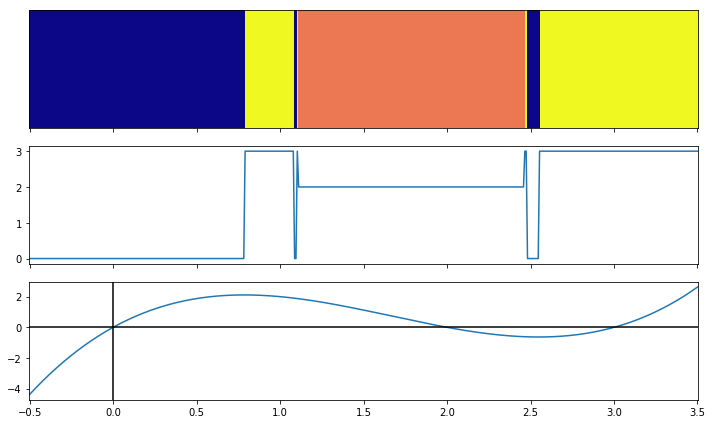
\includegraphics[width=4in]{images/newt1.png}
	\end{center}
	
	\newpage
	Zooming in around $x\approx 2.4588$:

	\begin{center}
	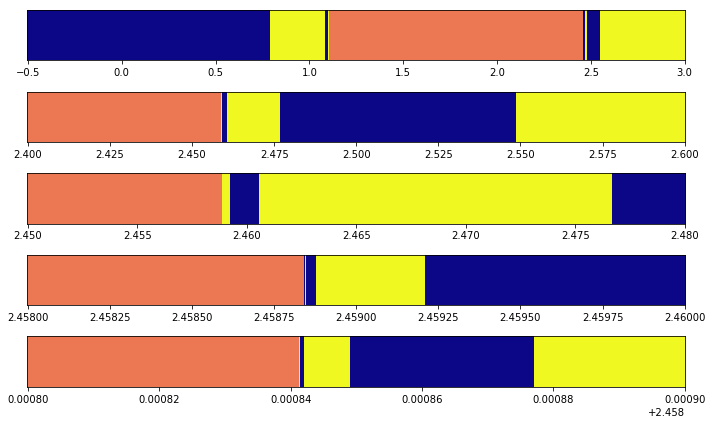
\includegraphics[width=4in]{images/newt2.png}
	\end{center}

	We've just seen our first {\bf fractal}! For now, we will define a \emph{fractal}
	as a set with repeated patterns at all scales.

	\newpage
	\section*{Fractals}
	Let's construct some famous fractals.

	\question
	Let $K_0$ be an equilateral triangle with sides of length $1$. 
	Let $K_1$ be the result
	of applying 
	\mbox{
	\begin{tikzpicture}[scale=.6]
		\draw[blue, thick] (0,0)--(1,0);
	\end{tikzpicture} $\to$ 
	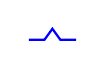
\begin{tikzpicture}[scale=.6]
		\draw[blue, thick] (0,0)--(1/3,0) -- (1/2, .23) -- (2/3, 0) -- (1,0);
	\end{tikzpicture}} to each side of $K_0$. Repeat this process to get $K_2$ from $K_1$, etc. and define
	\[
		K_{\infty} = \lim_{n\to\infty} K_n.
	\]
	\begin{parts}
		\item Draw $K_0$, $K_1$, and $K_2$.
		\item Find the perimeter of $K_0$, $K_1$, and $K_2$. Find a general
			formula for the perimeter of $K_n$.
		\item What is the perimeter of $K_{\infty}$? What is the area enclosed by
			$K_{\infty}$?
	\end{parts}
	$K_\infty$ is called the \emph{Koch Snowflake}.

	\question
	Let $T_0$ be a filled-in equilateral triangle. To get $T_1$, $T_2$, etc., apply the substitution
	rule
	\mbox{
	
\begin{tikzpicture}[scale=.6]
		\fill[blue, thick] (0,0)--(1,0) -- (.5, .866);
	\end{tikzpicture} $\to$ 
	
\begin{tikzpicture}[scale=.6, even odd rule]
		\fill[blue, thick] (0,0)--(1,0) -- (.5, .866)  (.5,0) -- (1/4,.433) -- (3/4, .433);
	\end{tikzpicture}} to each (sub)triangle of $T_0$, $T_1$, etc..  Define $T_{\infty}$ to be the limit
	of this process.
	\begin{parts}
		\item Draw $T_0$, $T_1$, and $T_2$.
		\item Find a formula for the area of $T_n$.
		\item Compute the area of $T_\infty$.
		\item Is $T_\infty$ the empty set? Why or why not?
	\end{parts}
	$T_\infty$ is called \emph{Sierpinski's Triangle}.

	\question
	Let $C_0=[0,1]$ be the unit interval. Recursively define $C_i$ by the substitution
	rule 
	\mbox{
	\begin{tikzpicture}[scale=.6]
		\draw[blue, thick] (0,0)--(1,0);
	\end{tikzpicture} $\to$ 
	\begin{tikzpicture}[scale=.6]
		\draw[blue, thick] (0,0)--(1/3,0)  (2/3, 0) -- (1,0);
	\end{tikzpicture}}, which removes the middle $1/3$ of every interval. 
	Define $C_\infty$ to be the limit of this process.


	\begin{parts}
		\item Compute the length of $C_n$.
		\item Compute the length of $C_\infty$.
	\end{parts}
	$C_\infty$ is called the \emph{Cantor set}.


	\bigskip
	Our normal sense of measurement fails when it comes to these fractals. We need a new idea: \emph{similarity dimension}.

	\newpage
	\subsection*{Dimension}

	Dimension can be thought of as a relationship between scale and content\footnote{Here ``content'' refers to the ``stuff inside'' of an object.}.

	\question
	\begin{parts}
		\item 
		Let $\ell=[0,1)$, $2\ell=[0,2)$, $3\ell=[0,3)$, etc.. How many disjoint copies of $\ell$ does it take to
		cover $n\ell$?
		\item Let $S=[0,1)^2$, $2S=[0,2)^2$, etc.. How many disjoint copies of $S$ does it take to cover $nS$?
		\item Let $C=[0,1)^3$, $2C=[0,2)^3$, etc.. How many disjoint copies of $C$ does it take to cover $nC$?
		\item Based on the patterns you see, describe an algorithm that can be used to find the dimensions of $\ell$, $S$, and
			$C$.
		\item Let $T$ be the filled-in equilateral triangle. Apply your algorithm to $2T$.
		\item Let $T_\infty$ be the Sierpinski triangle. Apply your algorithm to $2T_\infty$. Does the number you get
			make sense?
	\end{parts}

	\begin{definition}[Similarity Dimension]
		A set $Q\subseteq \R^n$ has \emph{similarity dimension} $d$ if there exists a $c\in \Z$
		and $s\in \R_{\geq 1}$ satisfying
		\[
			d=\log_s(c)
		\]
		and $sQ$ ($Q$ scaled up by a factor of $s$) is covered by
		$c$ copies of $Q$ (at most overlapping on their boundaries).

	\end{definition}

	\question
	\begin{parts}
		\item Compute the similarity dimension of a (a) a line segment, (b) the Cantor set, and (c) Sierpinski's triangle.
		\item Compute the similarity dimension of the Koch snowflake.
	\end{parts}

	What about sets that aren't self-similar? 

	\question
	Let $K_\infty'$ be the ``Koch snowflake'' obtained with the substitution rule
	\mbox{
	\begin{tikzpicture}[scale=.6]
		\draw[blue, thick] (0,0)--(1,0);
	\end{tikzpicture} $\to$ 
	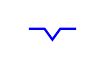
\begin{tikzpicture}[scale=.6]
		\draw[blue, thick] (0,0)--(1/3,0) -- (1/2, -.23) -- (2/3, 0) -- (1,0);
	\end{tikzpicture}}.

	\begin{parts}
		\item Find the perimeter and dimension of $K_{\infty}'$.
		\item Let $K_{\text{strange}}$ be the ``Koch snowflake'' obtained by 
		the rule \mbox{
			\begin{tikzpicture}[scale=.6]
				\draw[blue, thick] (0,0)--(1,0);
			\end{tikzpicture} $\to$ 
			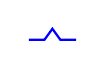
\begin{tikzpicture}[scale=.6]
				\draw[blue, thick] (0,0)--(1/3,0) -- (1/2, .23) -- (2/3, 0) -- (1,0);
			\end{tikzpicture} or 
			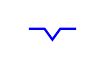
\begin{tikzpicture}[scale=.6]
				\draw[blue, thick] (0,0)--(1/3,0) -- (1/2, -.23) -- (2/3, 0) -- (1,0);
			\end{tikzpicture}
			} chosen randomly at each stage.
		What should the dimension of $K_{\text{strange}}$ be? Can you compute it's similarity dimension?
	\end{parts}

	\newpage
	We need a way to define dimension for shapes that aren't self-similar. Let's again work from
	sets whose dimension we know: cubes.

	\begin{definition}[Box Covering]
		A $d$-dimensional \emph{box covering} of $X\subseteq \R^k$ is a collection $C=\Set{B_i}$ of 
		$d$-dimensional cubes which satisfy
		\begin{enumerate}
			\item if $i\neq j$, $B_i$ and $B_j$ intersect at most on their boundaries;
			\item $B_i\cap X\neq \Set{}$ for all $i$;
			\item $X\subseteq \bigcup_{i} B_i$.
		\end{enumerate}
	\end{definition}

	\begin{definition}[Outer Measure]
		The \emph{$d$-dimensional outer measure} of $X\subseteq \R^k$ is
		\[
			\lim_{n\to\infty} \inf_{C_n}\  \text{volume}(C_n)
		\]
		where $C_n$ is a $d$-dimensional box covering of $X$ with cubes of side-length $1/n$.
	\end{definition}
	You should think of $\inf_{C_n}\  \text{volume}(C_n)$ as the ``smallest possible box covering of size $1/n$ that
	still covers the set''.

	\question
	Let $\ell\subseteq \R^3$ be the line segment from $\vec 0$ to $(1,0,0)$.
	\begin{parts}
		\item Find the $1$, $2$, and $3$-dimensional outer measures of $\ell$.
		\item Does $\ell$ have a $0$-dimensional outer measure?
		\item Let $T\subseteq \R^3$ be the filled in triangle with vertices $(0,0,0)$, $(1,0,0)$,
			and $(0,1,0)$. Find the $1$, $2$, and $3$-dimensional outer measures of $T$.
		\item Find the $1$-dimensional outer measure of the Cantor set.
	\end{parts}

	\newpage
	What would it mean to have a fractional-dimensional outer measure? Let $B$ be a $d$-dimensional
	box with side lengths $k$. Its volume is $k^d$. Divide the box in half along every dimension and 
	each sub-box has volume $(k/2)^d=(1/2)^dk^d$, and so there must be $2^d$ sub-boxes.

	What if there were fewer ``sub-boxes''?

	\question
	Let $C_\alpha$ be the Cantor-like set obtained by removing the middle $\alpha$ of each subinterval.
	(I.e., the standard Cantor set is $C_{1/3}$.)
	\begin{parts}
		\item Find the number of boxes in a $1$-dimensional box-covering of $C_{0}$ 
			(the interval) and  $C_{1/3}$ where the width of each box is $1/3$, $1/9$, $1/27$, etc..
		\item Based on what you know about how many width-$k$ boxes it takes to fill $d$-dimensional space,
			find a formula relating $d$, the number of boxes, and the width of the boxes.
		\item Use your formula to estimate $d$ for $C_{1/3}$. How does this compare to the similarity-dimension
			of $C_{1/3}$?
	\end{parts}

	\begin{definition}[Box-counting Dimension]
		Let $X\subseteq \R^m$ and let $B\subseteq \R^m$ and let $B$ be a minimal-dimensional, minimally-sized box such
		that $X\subseteq B$. The \emph{box-counting dimension} of $X$ is
		\[
			d=\lim_{n\to\infty} \frac{\log(\text{\# of sub-boxes of $B_n$ that intersect $X$})}{\log n},
		\]
		where $B_n$ is $B$ ``cut'' along each axis into $n$ equally-spaced slices.
	\end{definition}

	\begin{parts}[resume]
		\item Find the box-counting dimension of $C_{1/3}$.
		\item Find the box-counting dimension of the unit simplex in $\R^2$. I.e. $\Set{\vec v\in \R^2\given \vec v=
			\alpha\xhat+\beta \yhat\text{ for some }\alpha,\beta\geq 0\text{ satisfying }\alpha+\beta \leq 1
			}$
		\item Intuitively, what should $\lim_{\alpha\to 0} \dim(C_\alpha)$ be? Find the box-counting and similarity
			dimension of $C_\alpha$ and verify.
	\end{parts}
	
	Box-counting dimension is difficult to compute exactly, but it's useful for approximations. Computers are
	pretty good at counting boxes!

	\newpage
	\subsection*{Markov Chains}
	
	\begin{definition}[Transition Matrix]
		Let $\mathcal G$ be a directed graph with vertices $\Set{1,\ldots, n}$.
		A \emph{transition matrix} for $\mathcal G$ is an $n\times n$ matrix $A=[a_{ij}]$ where
		\[
			a_{ij} = \begin{cases}
				1 &\text{ if there is an edge from $j$ to $i$}\\
				0 &\text{ otherwise}
			\end{cases}.
		\]
	\end{definition}

	\question
	The map shows the direct, one-way flights offered by the Pacific
	Rim air shipping company.
	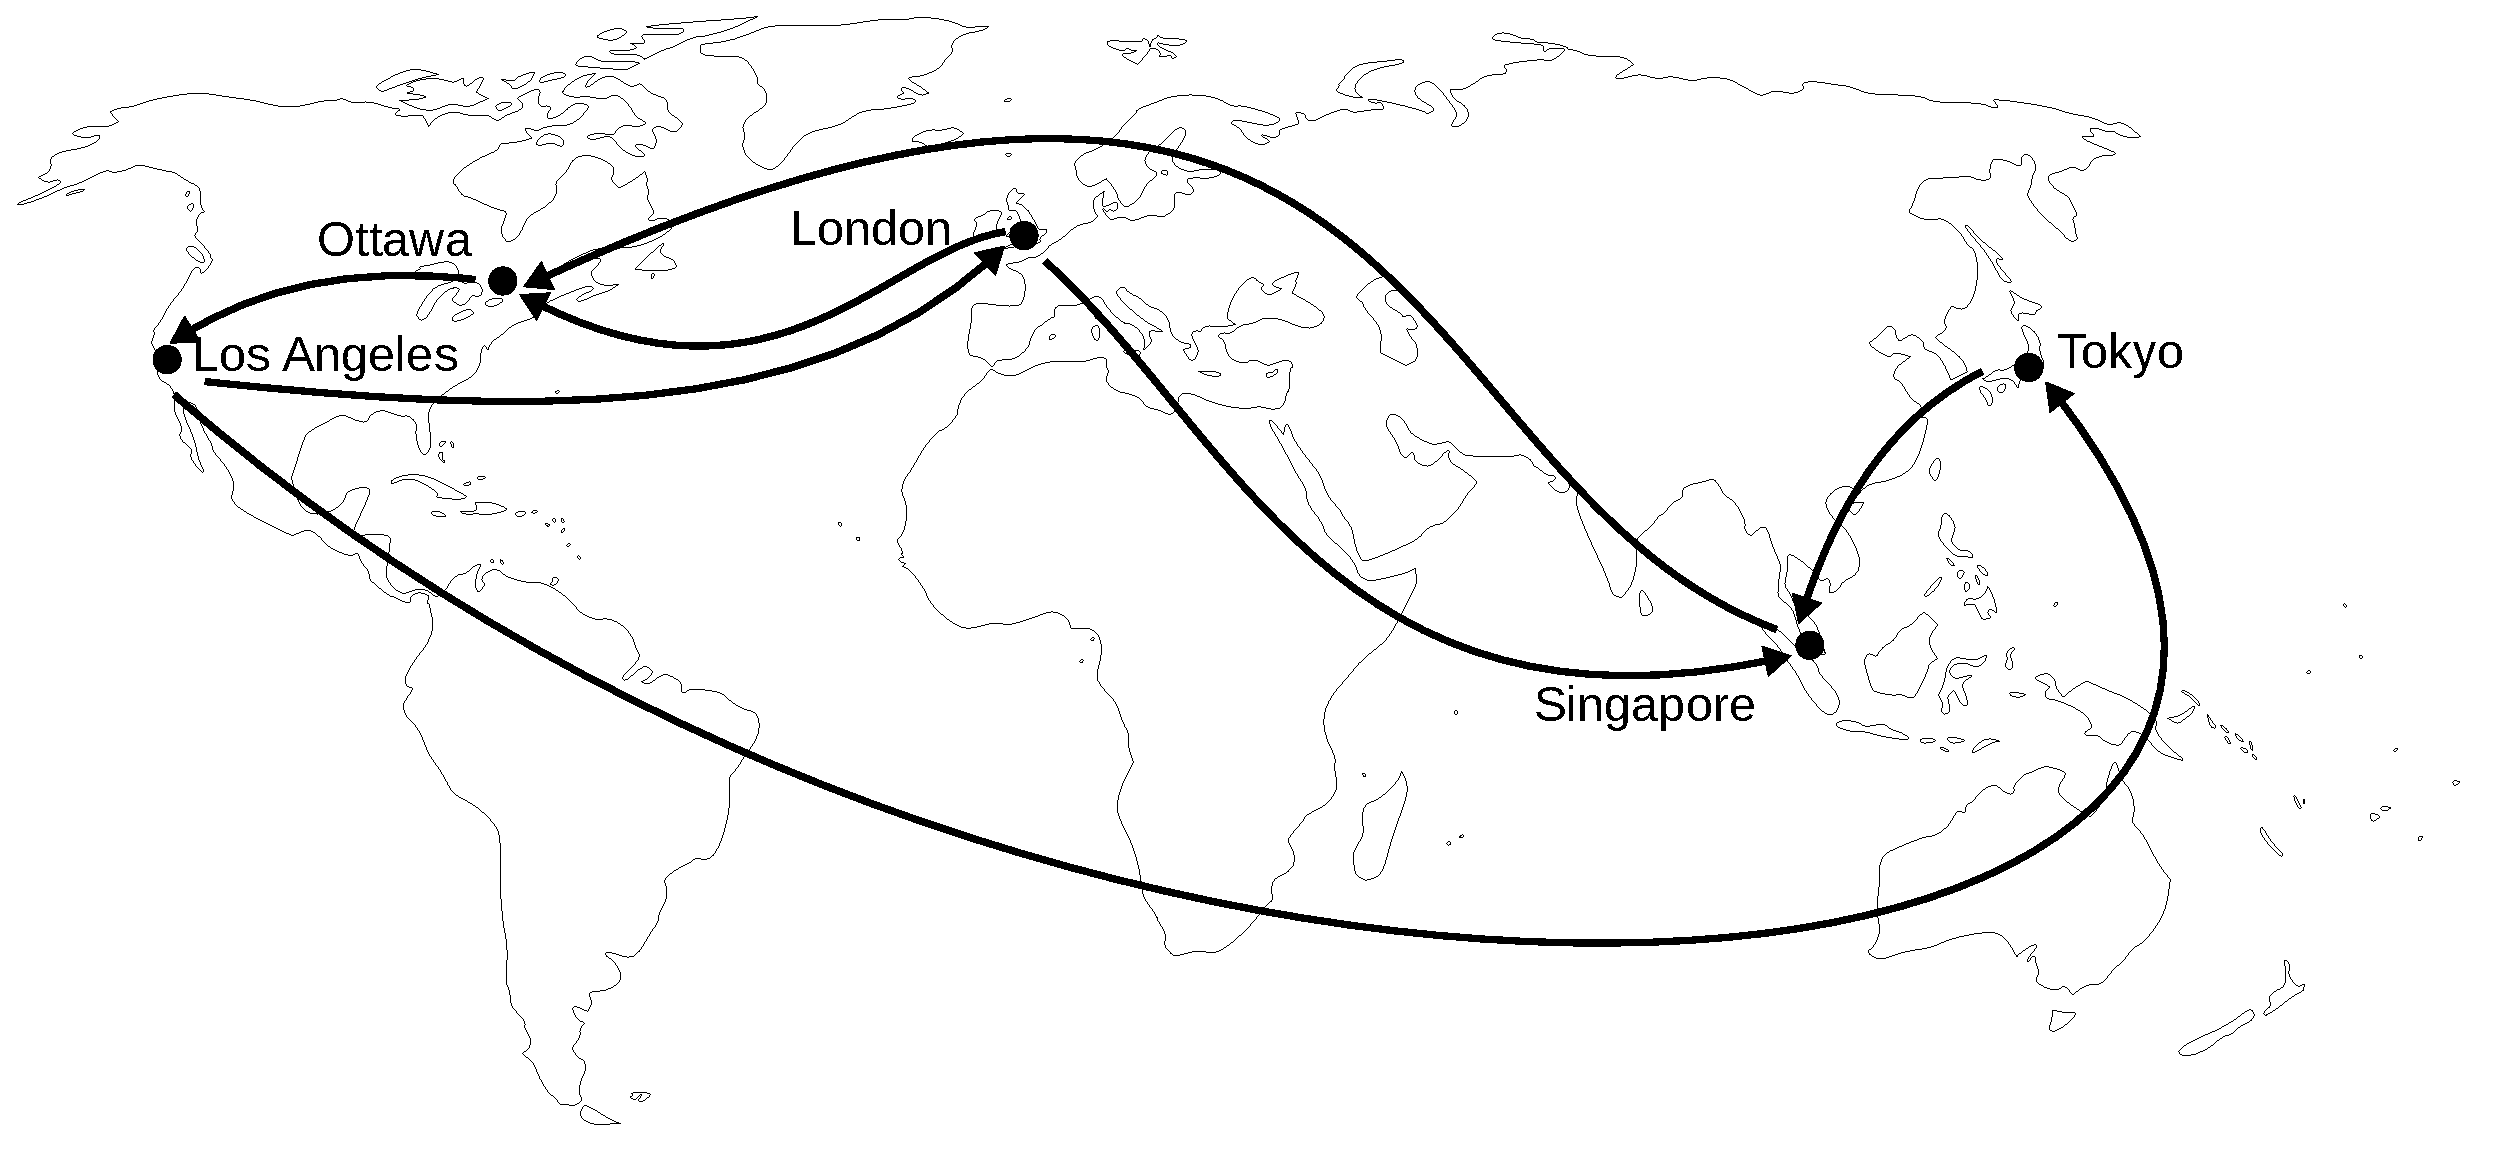
\includegraphics[height=2.5in]{images/flight_map.pdf}
	We can think of their flight map as a graph (in the graph-theory sense).


	\begin{parts}
		\item Write down a \emph{transition matrix} $A$ for the above graph.
		\begin{enumerate}
			\item What do the diagonal entries tell you about the available flights?
			\item Should $a_{ij} = a_{ji}$? Explain.
		\end{enumerate}
		\item Write down a matrix $B=[b_{ij}]$ where the entry $b_{ij}$ indicates the 
		number of ways to take exactly two flights from city $i$ to city $j$.
		\begin{enumerate}
			\item Compute $A^2$ and compare with $B$.
			\item What information does the $1$st row of $A$ give you about flights?
			\item What information does the $2$nd column of $A$ give you about 
			flights?
			\item Based upon your last two answers what does the $1,2$ entry of 
			$A^2$ tell you about flights?
		\end{enumerate}
		\item Compute $A^3$. What does it tell you about shipping routes?
		\item A package with a lost tracking number is getting kicked around from route to route!
			Each time it lands, it is randomly (and with equal probability)
			put on another flight.
			After several weeks (and 100s of flights), the package is finally noticed.
				Where is it most likely to be?
	\end{parts}


	\newpage
	\begin{definition}[Markov Chain]
		Given a graph $G$, a \emph{stationary Markov chain on $G$}, is a random process,
		denoted $X_1,X_2,\ldots$ where $X_i$ indicates the location on the graph at the $i$th
		step and the probability distribution of $X_i$ is {\it completely determined} by the value
		of $X_{i-1}$.
	\end{definition}
	Some people call stationary Markov chains ``memoryless'' processes because what happened more than one
	step prior has no affect on what happens in the next step.

	\question
	Consider the following directed graph with transition probabilities labeled.
	\begin{center}
	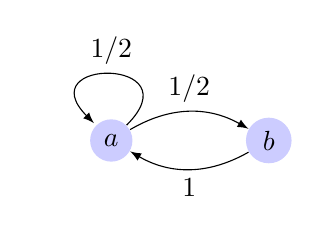
\begin{tikzpicture}[mainnode/.style={circle,fill=blue!20,minimum size=1em,inner sep=3pt]}]

	    \node[mainnode] (1) at (0,0) {$a$};
	    \node[mainnode] (2) at (2, 0)  {$b$};

		\path (1) edge[->, loop] node[above] {1/2} (1) 
		(1) edge[->, bend left] node[above] {1/2}(2) 
		(2) edge[->, bend left] node[below] {1}(1);
	\end{tikzpicture}
	\end{center}

	\begin{parts}
		\item Find a transition matrix, $T$, for the graph.
		\item Find a matrix $P_1$ whose $i,j$ entry represents the probability
			of transitioning from state $j$ to state $i$ in exactly one step.
		\item Find a matrix $P_2$ whose $i,j$ entry represents the probability
			of transitioning from state $j$ to state $i$ in exactly two steps.
		\item How do $P_2$ and $P_1^2$ relate?
		\item Does $\lim_{n\to\infty} P_1^n$ exist? If so, what is it?
	\end{parts}

	\begin{definition}[Stochastic Matrix]
		A vector $\vec v\in \R^n$ is called a \emph{probability vector} if its entries are non-negative and sum to
		one. A matrix is called a \emph{stochastic matrix} if its columns are probability vectors.
	\end{definition}

	In the context of Markov chains, we also refer to stochastic matrices as \emph{transition} matrices\footnote{ Yes, this word
	is doing double duty!}.

	\question
	You're a picky eater. You have meals of healthy food and dessert, but you never have healthy food twice in a row.
	Each time you eat dessert, you flip a weighted coin to decide what meal to eat next. Let $p$ represent the weight of
	the coin.
	\begin{parts}
		\item Are your eating habits described by a Markov chain? Why or why not?
		\item Draw a graph representing this situation.
		\item Your friend visits you for New Years and sees your having a healthy dinner. You lose touch
			after that, but bump into each other at a restaurant six years later. What type of meal are
			you most likely to be eating? Does this depend on $p$?
	\end{parts}

	\question
	\begin{parts}
		\item Is a Markov chain a dynamical system? Why or why not?
		\item Consider the Markov chain with states $\Set{a,b}$
			given by the transition matrix $\mat{1/2&1\\1/2&0}$. Given 
			that you start in state $a$, give probability vectors indicating the 
			probability of being in a particular state after $0$, $1$, $2$, and $3$ steps
			along the Markov chain.
		\item Can this Markov chain be \emph{modeled} by a dynamical system? If so, describe
			such a model.
	\end{parts}

	\newpage
	\subsection*{Iterated Function Systems (IFS)}

	\begin{definition}[Realization of a Markov Chain]
		Given a Markov Chain $\mathcal M = (X_1,X_2,\ldots)$ with state space $S$, a \emph{realization} 
		of $\mathcal M$ is a sequence of states whose transitions are allowed by the Markov chain. I.e.,
		an allowed element of $S^{\N}$.

		A realization $\vec r\in S^{\N}$ is called \emph{generic} for $\mathcal M$
		if the transition probabilities for $\mathcal M$ can be recovered from $\vec r$ by
		averaging.
	\end{definition}
	
	\question
	Consider the Markov chain $\mathcal M$ with state space $[0,1]$ and the transition rule
	\[
		X_{i+1} =\begin{cases}
			X_i/3 &\text{ with probability $1/2$}\\
			X_i/3 + 2/3 &\text{ with probability $1/2$}
		\end{cases}
	\]
	\begin{parts}
		\item Using a random number generator, write down the initial segment (up to 4 transitions) of two
		different realizations of $\mathcal M$.
		\item Let $\vec r=(r_0,r_1,\ldots)$ be a realization of $\mathcal M$. Is it possible that
			$\lim_{i\to\infty} r_i$ exists? Why or why not?
		\item Let $\vec s=(s_0,s_1,\ldots)$ be a realization for $\mathcal M$ that is generic. 
			Is it possible that
			$\lim_{i\to\infty} s_i$ exists? Why or why not?
		\item Can $\mathcal M$ be modeled by a dynamical system? If so, describe the model.
		\item Suppose we start off with a uniform distribution on $[0,1]$. Draw the
			resulting distribution after $1$, $2$, and $3$ steps along $\mathcal M$. 
	\end{parts}

	\newpage
	\begin{definition}[Iterated Function System (IFS)]
		An \emph{iterated function system} with functions $(f_1,\ldots,f_n)$
		and transition probabilities $(p_1,\ldots,p_n)$ 
		is a stationary Markov chain where transitions are given by the rule
		\[
			X_{i+1} =
			\begin{cases}
				f_1(X_i) &\text{ with probability $p_1$}\\
				f_2(X_i) &\text{ with probability $p_2$}\\
				& \vdots 
			\end{cases}
		\]
	\end{definition}

	\begin{definition}[Invariant Set]
		Let $\mathcal I$ be an iterated function system with functions 
		$(f_1,\ldots,f_n)$ and non-zero transition probabilities $(p_1,\ldots,p_n)$.
		The set $X$ is called an \emph{invariant set} for $\mathcal I$ if
		\[
			X=\bigcup_i f_i(X).
		\]
	\end{definition}

	\question
	Let $\mathcal I$ be the iterated function system with transition probabilities $(1/2,1/2)$
	and functions $(f_1:[0,1]\to[0,1],f_2:[0,1]\to[0,1])$ given by
	$f_1(x)=x/3$ and $f_2(x)=x/3+2/3$.
	\begin{parts}
		\item Find an invariant set for $\mathcal I$.
		\item Is the Cantor set an invariant set for $\mathcal I$?
		\item Is there a larger invariant set for $\mathcal I$ than the Cantor set? Why or why not?
		\item If the probabilities for $f_1$ and $f_2$ change, will that affect the invariant sets?
	\end{parts}

	\question
	Define $f_{\vec a}:[0,1]^2\to[0,1]^2$ by $f_{\vec a}(\vec x)=\vec x/2 + \vec a$. Let $\mathcal F$ be
	the iterated function system with functions $(f_{\vec 0}, f_{(1/2,0)}, f_{(0,1/2)})$ and equal probabilities.
	\begin{parts}
		\item Draw a maximal invariant set for $\mathcal F$.
		\item Can you create an iterated function system so that the Sierpinski triangle is
			an invariant set? If so, do it!
	\end{parts}


	\newpage
	\subsection*{Continuous-time Dynamical Systems}
	The dynamical systems we've seen so far involve taking one ``step'' at a time.
	However, as we experience life, it seems like time advances continuously, not discretely.
	Can we capture that in a dynamical system?

	\begin{definition}[Continuous-time Dynamical System]
		Let $X$ be a set and let $(T^a:X\to X)_{a\in \R}$ be a family of functions
		satisfying $T^a\circ T^b=T^{a+b}$. Then, $(T^a,X)$ is called a \emph{continuous time
		dynamical system}.
	\end{definition}

	\question
	\begin{parts}
		\item Let $S^a:\R\to\R$ be defined by $S^a(x)=ax$. Is $(S^a,\R)$ a continuous time dynamical system?
		\item Let $T^a:\R\to\R$ be defined by $T^a(x)=2^a x$. Is $(T^a,\R)$ a continuous time dynamical system?
		\item Let $\mathcal F=\Set{\text{functions from $\R$ to $\R$}}$ and define $E^t:\mathcal F\to\mathcal F$
			by $E^t(f(x)) = f(x+t)$. Is $(E^t,\mathcal F)$ a continuous time dynamical system?
	\end{parts}

	\newpage
	\question
	\begin{parts}
		\item 

		Consider the following garden paths.
		\begin{center}
			
\includegraphics[width=2in]{images/garden-path.pdf}
		\end{center}
		Let $P$ represent the set of points on the paths and define $W^t:P\to P$ to be the result of walking
		at unit speed counter-clockwise around your path for $t$ seconds.

			Is $(W^t,P)$ a continuous time dynamical system?

		\item You're watching the surface of a lake and carefully map out the velocity of the
			water at each point. You produce the following picture of velocities.
		\begin{center}
			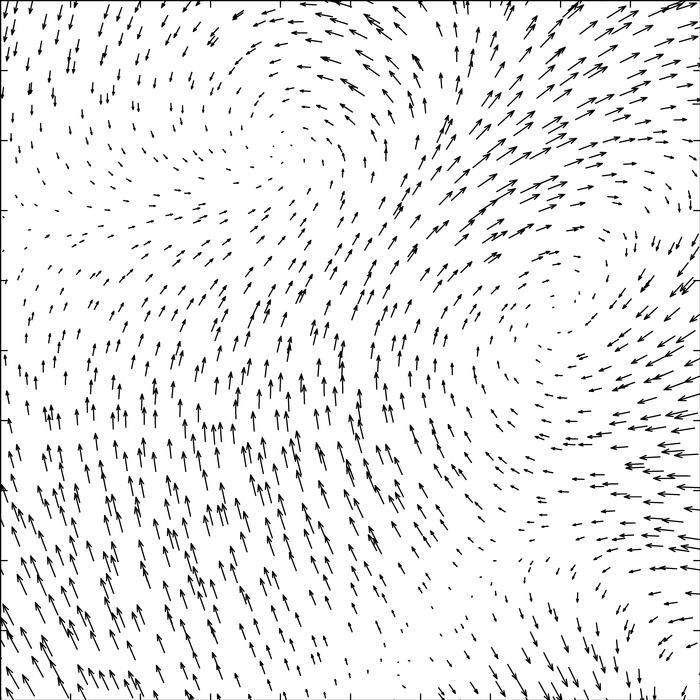
\includegraphics[width=3in]{images/vectorfield1.jpg}
		\end{center}
			Let $S$ be the points on the surface of the lake and let $\Phi^t:S\to S$ be the result
			of ``flowing'' along the surface for $t$ seconds. Is $(\Phi^t, S)$ a continuous time dynamical system?
	\end{parts}

	Systems like $(\Phi^t,S)$ come up often because they are described by \emph{local} rules. That is, recorded in the
	picture is information about where you flow after tiny time increments---finding where you end up after bigger time
	increments takes work.

	\newpage
	\begin{definition}[Vector Field]
		Given a set $X$, a \emph{$n$-dimensional vector field on $X$} is a function $F:X\to \R^n$ which
		assigns a vector to each point in $X$.
	\end{definition}

	Vector fields show up a lot in physics because \emph{velocities} and \emph{accelerations} of particles in a fluid
	naturally produce vector fields.

	\question
		Let $V:\R^2\to\R^2$ be a vector field and let $\Phi^t:\R^2\to\R^2$ be the function which ``flows'' points along
		the vector field with velocity at a given point equal to the vector at that point.
	\begin{parts}
		\item Find a $V$ so that all points flow vertically at unit speed.
		\item Find a $V$ so that all points flow radially outward and increase in speed.
		\item Find a $V$ so that all points flow around in a circle.
		\item Find a $V$ so that all points flow around in a circle at the same speed.
		\item Find a $V$ so that all points flow around in a circle with the same period (that is, it takes the same
			amount of time for any given point to go around the circle).
	\end{parts}

	\begin{definition}[Flow \& Orbit]
		Let $(W^t,X)$ be a continuous time dynamical system and let $x\in X$. 
		The \emph{flow of $W^t$ starting at $x$} is the function $f:\R\to X$ defined by
		\[
			f(t) = W^t(x).
		\]
		The \emph{orbit of $x$ under $W^t$} is the set $\Set{f(t):t\in \R}$, where $f$ is the flow of $W^t$
		starting at $x$. We call the set $\Set{f(t):t\in \R^+}$ the \emph{forward orbit} of $x$.
	\end{definition}
	We will often notate the flow of $W^t$ starting at $x$ by $\phi_t(x)$. As a flow, we think of $t$ as the variable.

	\question
		Let $V:\R^2\to\R^2$ be a vector field and let $\Phi^t:\R^2\to\R^2$ be the function that flows
		points along the vector field. 
	\begin{parts}
		\item If possible, find a $V$ so that some orbits are infinitely long.
		\item If possible, find a $V$ so that some orbits are not infinitely long.
		\item If possible, find a $V$ so that some orbits are infinitely long and others are not.
		\item If possible, find a $V$ so that all orbits are finite line segments.
		\item If possible, find a $V$ so that the forward orbit of every point ends up at $\vec e_1$.
		\item If possible, find a $V$ so that the forward orbit of every point ends up at $\vec 0$ or $\vec e_1$ (and
			at least one orbit heads towards $\vec 0$ and one towards $\vec e_1$).
	\end{parts}

	\newpage
	\begin{definition}[Stable \& Unstable Points]
		Let $(W^t,\R^n)$ be a continuous time dynamical system and let $\phi_t(\vec w)$
		represent the flow of $W^t$ starting at $\vec w\in\R^n$. We call the point $\vec x\in \R^n$ \emph{stable}
		if for all $\varepsilon>0$, there exists a $\delta>0$ so that for all $\vec y\in \R^n$, 
		\[
			\Norm{\vec x-\vec y} < \delta\qquad \text{implies}\qquad
		\Norm{\phi_t(x)-\phi_t(y)} < \varepsilon \qquad \text{ for all }\qquad t > 0.
		\]
		Otherwise, $\vec x$ is called \emph{unstable}.
	\end{definition}

	\question
	Given a $2\times 2$ matrix $M$, define a vector field $V_M:\R^2\to\R^2$ by $V_M(\vec x)=M\vec x$. Consider the following matrices
	and their associated vector fields:
	\[
		I=\mat{1&0\\0&1}\quad
		A=\mat{-1&0\\0&-1}\quad
		B=\mat{0&-1\\1&0}\quad
		C=\mat{1&-1\\1&1}\quad
		D=\mat{-1&-1\\1&-1}\quad
		E=\mat{0&1\\1&0}
	\]
	\begin{parts}
		\item Explain in plain language what it means for $x$ to be a \emph{stable} point of a continuous
			dynamical system.
		\item Use an online plotter (for example \url{https://www.desmos.com/calculator/eijhparfmd} or
			\url{https://anvaka.github.io/fieldplay}) to
			plot $V_X$ for $X\in\{I,A,B,C,D,E\}$ and determine which points are stable/unstable for each.
		\item Compute the eigenvalues for each of the matrices. Can you relate the eigenvalues to 
			stable/unstable points?
	\end{parts}

	\newpage
	\subsection*{Differential Equations}
	To really get a handle on what's going on, let's think about some differential equations!

	\question
	\begin{parts}
		\item Let $a$ be a constant. Find a non-trivial solution to the differential equation $f'(t)=af(t)$.
		\item Consider the (boring) vector field $V:\R^1\to\R^1$ defined by $V(t)=at$. Find a non-trivial flow
			for the corresponding dynamical system. Is $V$ given by matrix multiplication? If so, what's the matrix?
		\item Let $D=\mat{a&0\\0&b}$ and define the vector field $W:\R^2\to\R^2$ by $W(\vec x)=D\vec x$. Find a non-trivial
			flow for the corresponding dynamical system.

			Can you give conditions on $a$ and $b$ so that $\vec 0$ is stable/unstable with respect to the corresponding
			dynamical system? If $a$ and $b$ are complex numbers, does that change your answer?
		\item Suppose $(W^t,\R^n)$ is a continuous dynamical system. Define what the \emph{derivative of $W^t$ with respect to
			time} should mean. How does this relate to vector fields and flows?
		\item Prove that if $f:\R\to\R^n$ is a function and $M$ is a matrix, then $(Mf)'=M(f')$.
		\item Suppose $A$ is a matrix and $A=PDP^{-1}$ where $D$ is diagonal. Further,
			suppose $f$ is a solution to $f'(t)=Df(t)$. Find a solution to the differential equation
			$\Phi'(t)=A\Phi(t)$.
		\item Let $M$ be a matrix and consider the continuous dynamical system coming from the vector field $\vec x\mapsto M\vec x$.
			Classify the behaviour near $\vec 0$ based on the eigenvalues of $M$.
	\end{parts}

	\question
	\label{QCTS}
	Consider the continuous dynamical systems $(W^t_1,\R^2)$, $(W^t_2,\R^2)$, $(W^t_3,\R^2)$, and $(W^t_4,\R^2)$
	given by flows along the vector fields
	\[
		V_1\mat{x\\y}=\mat{-y\\x}\qquad
		V_2\mat{x\\y}=\matc{x+y^2\\-y}\qquad
		V_3\mat{x\\y}=\matc{-y\\x+y^2}\qquad
		V_4\mat{x\\y}=\matc{-x+y^2\\-y}
	\]
	\begin{parts}
		\item Classify $(0,0)$ as stable or unstable for each system.
		\item Classify $(0.01,0.01)$ as stable or unstable for each system.
		\item Conjecture: under what conditions will a first-order approximation about at a
			fixed point tell you about stability \emph{near} that fixed point.
			\label{QCTS:b}
	\end{parts}

		
	\begin{definition}[Structural Stability]
		A continuous dynamical system $(W^t,X)$ is called \emph{structurally stable at $\vec x\in X$
		with respect to fixed points/stable points/periodic points/etc.} if the topology of
		the set of fixed points/stable points/periodic points/etc. near $\vec x$ remains invariant with respect
		to small perturbations of $W^t$.
	\end{definition}

	\question
	\begin{parts}
		\item What should a \emph{small perturbation} of $(W^t,\R^n)$ mean?
		\item What should it mean for the \emph{topology} of a set to be \emph{invariant}?
		\item Out of the examples in \ref{QCTS}, which are structurally stable at $\vec 0$?
		\item Revisit your conjecture from \ref{QCTS}.\ref{QCTS:b}. Can you rephrase it in terms of structural
			stability?
	\end{parts}

	\newpage
	\begin{definition}[Time-$1$ Map]
		Let $(W^t,X)$ be a continuous dynamical system. The \emph{time-$1$ map}
		associated with $(W^t,X)$ is the dynamical system $(T,X)$ where
		\[
			T(x) = W^1(x)
		\]
		for all $x\in X$.
	\end{definition}

	\question
	\label{QCIRCCONT}
	Let $S$ be a circle of circumference $1$ and let $(W^t_k,S)$ be the continuous dynamical
	system that flows points counter-clockwise along $S$ at speed $k$.
	\begin{parts}
		\item For which $k$ is the time-$1$ map associated with $(W^t_k,S)$ trivial?
		\item For which $k$ does the time-$1$ map associated with $(W^t_k,S)$ have periodic points?
	\end{parts}

	\newpage
	\subsection*{Circle Maps}
	Let $S$ be a circle of circumference $1$. We can associate $S$ with the unit interval $[0,1]$ provided
	we ``glue'' the endpoints together. We write $[0,1]/0\sim1$ to notate the set $[0,1]$ where $0$ and $1$
	are considered the same point. That is, if you move to the right starting at $0.99$, you'll wrap around
	and end up at $0.01$.

	Given a function $f:[0,1)\to\R$, we can create a function $g:[0,1)\to[0,1)$ via the formula
	\[
		g(x) = f(x)\mod 1.
	\]
	That is, compute the value $f(x)$ with ``wrap around'', and that's what $g(x)$ is.

	\begin{definition}[Symbolic Coding]
		Let $(T,X)$ be a discrete dynamical system and let $\mathcal P=\Set{P_a,P_b,\ldots}$
		be a partition of $X$. A \emph{symbolic coding} of $x\in X$ relative to the partition $\mathcal P$
		is the sequence 
		\[
			\C(x)=(c_0,c_1,\ldots)
		\]
		where
		\[
			c_i = \begin{cases}
				a &\text{ if }\quad T^ix\in P_a\\
				b &\text{ if }\quad T^ix\in P_b\\
				\,\vdots &
			\end{cases}
		\]
	\end{definition}


	\question
	Let $(W^t_k,S)$ be as in \ref{QCIRCCONT}. We can describe this dynamical system by
	\[
		W^t_k(x) = x+kt\mod 1.
	\]
	Let $P_a=[0,1/2)$ and $P_b=[1/2,1)$ be a partition of $[0,1]/0\sim 1$, and let $(T_k,S)$
	be the time-$1$ map for $(W^t_k,S)$.
	\begin{parts}
		\item Let $k=0.25$. Find $\C(0)$, $\C(1/5)$, and $\C(1/3)$ for $T_k,\{P_a,P_b\}$.
		\item Suppose $\C(x)=(a,a,b,b,a,a,b,b,\ldots)$. What can you say about $x$ and $k$?
		\item Is $(a,b,a,a,b,b,a,a,a,b,b,b,\ldots)$ the symbolic coding of any point? Why or why not?
		\item For which $k$ can $x$ be \emph{exactly} recovered from $\C(x)$?
		\item Let $\Set{a,b}^\N$ be the set of sequences of $a$'s and $b$'s. We can think
			of $\C:S\to\Set{a,b}^\N$ as a function. For which $k$ is $\C$ one-to-one? Onto?
	\end{parts}

	\newpage
	\subsection*{The Doubling Map}
	\begin{definition}[Orbit]
		Let $(T,X)$ be a discrete dynamical system. The \emph{orbit} of a point $x\in X$
		under $T$ is the set
		\[
			\mathcal O(x)=\Set{T^ix\given i\in\Z}
		\]
		if $T$ is invertible and 
		\[
			\mathcal O(x)=\Set*{T^ix\given i\in \N\cup\Set{0}}
		\]
		if $T$ is non-invertible.
	\end{definition}
	
	The \emph{doubling map} is the function $T:[0,1)\to[0,1)$ defined by $x\mapsto 2x\mod 1$.

	\question
	Let $\mathcal P=\Set{\mathcal P_0,\mathcal P_1} = \Set{[0,1/2),[1/2,1)}$ be a partition of $[0,1)$
	And let $\C:[0,1)\to\Set{0,1}^\N$ be the coding function arising from the doubling map and the partition $\mathcal P$.
	\begin{parts}
		\item Is the map $Q:\R\to\R$ defined by $x\mapsto 2x$ invertible? Is the doubling map invertible? Explain.
		\item Find $\mathcal O(1/3)$, $\mathcal O(4/5)$, and $\mathcal O(0)$ under the doubling map.
		\item Find $\C(1/3)$, $\C(4/5)$, and $\C(0)$.
		\item Suppose $\mathcal O(x)$ is a finite set. What can you say about $\C(x)$?
		\item Suppose $x\neq y$. Is it possible that $\C(x)=\C(y)$?
		\item Is $\C$ invertible?
		\item Define $\E:\Set{0,1}^\N\to[0,1)$ by \[
				(a_1,a_2,a_3,\ldots)\mapsto \sum \frac{a_i}{2^i}.
				\]
		Compute $\E(\C(1/2))$,  $\E(\C(1/3))$, and $\E(\C(4/5))$.
		\item What is $\E\circ \C$? How about $\C\circ \E$?
	\end{parts}

	\begin{definition}[Base-$n$ Expansion]
		A number $x\in [0,1)$ has a \emph{base-$n$ expansion} $0.d_1d_2d_3\cdots$ if
		\[
			x=\sum \frac{d_i}{n^i}.
		\]
	\end{definition}

	\question
	\begin{parts}
		\item Explain how base-$2$ representations relate to dynamical systems.
		\item Find a dynamical system and a partition so that $\C$ produces base-$10$ representations.
		\item Is the map from a number to its base-$n$ representation invertible? Explain.
	\end{parts}


	\newpage
	\subsection*{The Shift Space}

	\begin{definition}[Full Shift]
		Let $\Omega=\Set{0,1,\ldots,n-1}^\N$ and define $\sigma:\Omega\to\Omega$ by
		\[
			\sigma(a_0,a_1,a_2\ldots) = (a_1,a_2,\ldots).
		\]
		The dynamical system $(\sigma, \Omega)$ is called
		the \emph{full shift on $n$ symbols}. 
	\end{definition}

	The dynamical system $(\sigma, \Omega)$ is also called a \emph{shift space} and is equipped
	with a topology coming from the \emph{standard metric} on $\Omega$. This metric determines which
	sequences converge.

	\begin{definition}[Standard Metric on $\Omega$]
		The \emph{standard metric} on $\Omega$ is the function $d:\Omega\times \Omega\to[0,\infty)$ defined by
		\[
			d(x,y) = \begin{cases}
				0 & \text{ if }x=y\\
				2^{-i}&\text{ where } i=\min_j\Set{j:x_j\neq y_j}
			\end{cases}
		\]
		where $x=(x_0,x_1,\ldots)$ and $y=(y_0,y_1,\ldots)$ are points in $\Omega$.
	\end{definition}

	\question
	Let $(\sigma,\Omega)$ be the full shift on two symbols.
	\begin{parts}
		\item Let $x=(1,0,1,0,1,0,\ldots)$ and $y=(0,0,0,0,1,0,1,0,\ldots)$.
			Find $d(x,y)$, $d(\sigma(x),\sigma(y))$, $d(\sigma^2(x),\sigma^2(y))$, \ldots.
		\item Let $\vec 1 = (1,1,1,\ldots)$. Find points $a,b\in\Omega$ so that 
			\[
				d(\sigma^n(a),\vec 1)\nearrow 1
			\qquad\text{and}\qquad
				d(\sigma^n(a),\vec 1)\searrow 0.
			\]

		\item Let $(T,[0,1))$ be the doubling map and let $\C$ be the coding function
			for the partition $\Set{[0,1/2),[1/2,1)}$. You can view $\C$ as a function
			from $[0,1)\to\Omega$.

			For $t=1/3$, compute $\C(t)$, $\C\circ T(t)$, and $\sigma\circ \C(t)$. What
			do you notice? Will this always happen?
		\item Is $\C([0,1))\subseteq \Omega$ closed? (I.e., does it include all its limit points?)
		\item Let $t,t'\in[0,1)$ and let $a=\C(t)$ and $a'=\C(t')$.
			\begin{enumerate}
				\item If $d(a,a')$ is small, what can you say about $|t-t'|$?
				\item If $|t-t'|$ is small, what can you say about $d(a,a')$?
			\end{enumerate}
	\end{parts}

	\newpage
	The full $2$-shift isn't a perfect representation of the doubling map, but it's close! And, it
	turns out to be much easier to study.

	\begin{definition}[Subshift]
		Let $(\sigma,\Omega)$ be the full shift on $n$ symbols. The system $(\sigma, X)$ is
		called a \emph{subshift} provided
		\begin{enumerate}
			\item $X\subseteq \Omega$ is a closed set (i.e., it contains all its limit points); and
			\item $X$ is $\sigma$-invariant (i.e., $\sigma(X)=X$).
		\end{enumerate}
	\end{definition}

	\question
	Consider the circle rotation with $k=1/4$. Let $\mathcal O(0)$ be the \emph{orbit}
	of $0$ under this map, and define $X=\C(\mathcal O(0))$ with the usual partition.
	\begin{parts}
		\item Write down $X$.
		\item Is $(\sigma, X)$ a subshift?
		\item For each $x\in X$, find a corresponding $x'\in [0,1)$ so that
			$x=\C_T(x')$ where $\C_T$ is the coding with respect to the \emph{doubling map}
			and the standard partition.
		\item Can you model a circle rotation with the doubling map/subshift?
	\end{parts}

	\newpage
	\question
	Let $\mathcal M$ be the Markov chain with transition matrix $\mat{.5&1\\.5&0}$ and let
	$\mathcal M'$ be the Markov chain with transition matrix $\mat{.5&.9\\.5&.1}$.

	Let $X=\Set{\text{realizations of $\mathcal M$}}$ and let
	$X'=\Set{\text{realizations of $\mathcal M'$}}$.
	\begin{parts}
		\item Is $(\sigma, X)$ a subshift? Why or why not? What does $\sigma$ mean in terms of the original Markov chain?
		\item Is $(\sigma, X')$ a subshift? What does it ``look'' like?
		\item Let $Y$ be the set of \emph{generic} realizations of $\mathcal M$. Is $(\sigma, Y)$ a subshift?
	\end{parts}

	\newpage
	\begin{definition}[Word]
		Fix $\Omega=\Set{0,\ldots, n-1}^\N$.
		The finite list $w=(w_0,\ldots,w_{k-1})\in \Set{0,\ldots, n-1}^k$ is called a \emph{word of length $k$} in $\Omega$.

		If $x=(x_0,x_1,\ldots)\in \Omega$, we say that \emph{$x$ contains the word $w$} if for some $j$, 
		$w_i = x_{j+i}$ for all $i=0,\ldots,k-1$.

		If $X\subseteq \Omega$, we say \emph{$X$ contains the word $w$} if there exists $x\in X$ where
		$x$ contains the word $w$.
	\end{definition}

	\begin{definition}[Normalized Topological Entropy]
		Let $(\sigma, X)$ be a subshift of the full shift $(\sigma, \Omega)$. The \emph{normalized topological entropy}
		of $X$ is
		\[
			\mathcal H(X) = \lim_{k\to\infty}\frac{\log(\text{\# words of length $k$ in $X$})}{\log(\text{\# words of length $k$ in $\Omega$})}.
		\]
	\end{definition}

	\question
	Let $\mathcal C$ be the $3$-state Markov chain with transition matrix $\mat{1&1&1\\0&0&0\\1&1&1}$
	and let $X\subseteq \Set{0,1,2}^\N=\Omega$ be the set of realizations of $\mathcal C$ starting at $0$ or $2$.
	\begin{parts}
		\item Draw the graph associated with $\mathcal C$.
		\item Find the (normalized topological) entropy of $(\sigma, X)$.
		\item Find the (normalized topological) entropy of $(\sigma, \Omega)$.
		\item Draw $\E(X)$ as a subset of $[0,1]$. What is its fractal dimension?
	\end{parts}

	\newpage
	Entropy gives a way of classifying subshifts based on how ``big'' they are. This can be interpreted
	as how densely a subshift can store information.

	\question
	Let $\Omega=\Set{0,1}^\N$ and let $X\subseteq \Omega$ be the set of points with no two $1$'s in a row.
	\begin{parts}
		\item How many words of length $1,2,3,4$ are there in $\Omega$? How about in $X$?
		\item Is $(\sigma, X)$ a subshift? Why or why not?
		\item Can $(\sigma, X)$ be modeled by a Markov chain? If so, write down its transition matrix (not the stochastic one,
			the other one).
		\item How do $A$, $A^2$, $A^3$,\ldots relate to the number of words in $X$?
		\item Find the entropy of $(\sigma, X)$.
		\item If you wanted to transmit $n$ bits of information but you were only allowed to send subwords of $X$, how long of a subword
			would you need?
	\end{parts}

	\newpage
	Entropy relates to how much information you can get about a point by asking a series of questions.

	\question
	Let $C\subseteq[0,1]$ be the standard Cantor set. Every ``piece'' of $C$ has a left and a right. You are trying to locate a 
	point $x\in C$ by asking a series of questions like:
	\begin{itemize}
		\item Is $x$ in the left or right half of $C$?
		\item Is $x$ in the left or right half of the left/right half of $C$?

			~~~~\vdots
	\end{itemize}
	\begin{parts}
		\item What can you say about $x$ if you know
			\begin{enumerate}
				\item it's in the left half of $C$?
				\item it's in the left half of the left half of $C$?
				\item it's in the right half of the left half of the left half of $C$?
			\end{enumerate}
		\item Let $A_n=(a_1,\ldots, a_n)\in\Set{\text{left},\text{right}}^n$ be the answers to the first $n$ questions
			you ask.

			Given $A_n$, what is the maximum error you could have in guessing $x$?
		\item Playing the same game trying to find the point  $y\in [0,1]$, you ask a series of left-right questions and
			get a sequence of answers $A_n'$. Given $A_n'$ what is the maximum error you could have in guessing $y$?
		\item Let $E_n$ be the maximum error you have in guessing $x$ given the answers $A_n$
			and let $E_n'$ be the maximum error you have in guessing $y$ given the answers $A_n'$.
			Compute
			\[
				\lim_{n\to\infty} \frac{\log(E_n)}{\log(E_n')}.
			\]
		\item If you want to locate a point in $[0,1]$ with error less than $\varepsilon$, how many left-right
			questions do you need to ask?
		\item If you want to locate a point in $C$ with error less than $\varepsilon$, how many left-right
			questions do you need to ask?

	\end{parts}


	\newpage
	\question
	Let $X\subseteq \Omega=\Set{0,1,2}^\N$ be the set of all sequences without $1$'s.
	\begin{parts}
		\item Given that $w$ is a length-$n$ word in $X$, how many yes-no questions do you need
			to ask to determine $w$?
		\item Given that $w$ is a length-$n$ word in $\Omega$, how many yes-no questions do you need
			to ask to determine $w$?
		\item How does entropy relate to the number of yes-no questions needed to determine a word?
	\end{parts}

	\newpage
	\begin{definition}[Expansive]
		A dynamical system $(T,X)$ is \emph{expansive} at the point $x\in X$ if there exists $\varepsilon>0$
		such that for all $y\neq x$,
		\[
			d(T^nx,T^ny) > \varepsilon
		\]
		for some $n\geq 0$. The system $(T,X)$ is called \emph{expansive} if it is expansive at every point in $X$.
	\end{definition}
	\question
	\begin{parts}
		\item What's the difference between being expansive and not being \emph{stable}?
		\item Let $(T,S)$ be a circle rotation by $1/4$. Is $(T,S)$ expansive?
		\item Let $(\sigma, \Omega)$ be the full two-shift. Is $(\sigma, \Omega)$ expansive?
		\item Let $(T_f, \R)$ be the Newton's method map from the first day of class. Is $(T_f,\R)$
			expansive?
		\item Suppose $(T,X)$ is an expansive dynamical system.
		\begin{enumerate}
			\item Can $(T,X)$ have fixed points?
			\item Can $(T,X)$ have a periodic point?
			\item Can $(T,X)$ have an attracting point?
		\end{enumerate}
	\end{parts}



	\newpage
	\begin{definition}[Transitivity]
		Let $(T,X)$ be a dynamical system. The point $x\in X$ is called \emph{transitive}
		if $\overline{\mathcal O(x)}=X$. The system $(T,X)$ is called \emph{transitive}
		if there exists a transitive point in $X$.
	\end{definition}
	Here, $\overline{\mathcal O(x)}=X$ denotes the \emph{closure} of the orbit of $x$. That is,
	all points that are limits of points in $\mathcal O(x)$.
	
	\question
	\begin{parts}
		\item Let $(T_{1/4},S)$ be a circle rotation with angle $1/4$. Find $\overline{\mathcal O(0)}$.
			Is $(T_{1/4},S)$ transitive?
		\item Let $(T_{\sqrt{2}},S)$ be a circle rotation with angle $\sqrt{2}$. Find $\overline{\mathcal O(0)}$.
			Is $(T_{\sqrt{2}},S)$ transitive?
		\item Let $(\sigma, \Omega)$ be the full two-shift and let $x=10100100010000100\cdots$. What is 
			$\overline{\mathcal O(x)}$.
		\item Is $(\sigma,\Omega)$ transitive?
	\end{parts}

	\newpage
	\begin{definition}[Chaos]
		A dynamical system $(T,X)$ is called \emph{chaotic} if it is both expansive and transitive.
	\end{definition}
	\question
	\begin{parts}
		\item Let $(T_\theta, S)$ be a circle rotation with angle $\theta$. Is $(T_\theta, S)$ chaotic?
		\item Let $(\sigma, \Omega)$ be the full two-shift. Is $(\sigma, \Omega)$ chaotic?
		\item Let $(\sigma, X)$ be a subshift of the full two-shift. Is $(\sigma, X)$ chaotic?
	\end{parts}

	\newpage
	Chaos is a battle between order and disorder. Expansivity says close points eventually get far, so you cannot
	``approximate'' a chaotic system into the future. Transitivity says that points (and open neighborhoods in
	particular) get smeared all over the space.

	We see systems like this in nature, and have a \emph{theory of probability} that we use to describe unpredictable events.
	Can we do something similar to ``predict'' chaotic systems?

	\begin{definition}[Indicator Function]
		Given a set $A\subseteq X$, the \emph{indicator of $A$} is the function
		$\mathbb I_A:X\to\Set{0,1}$ defined by
		\[
			\mathbb I_A(x) = \begin{cases}
				1 &\text{ if $x\in A$}\\ 0 &\text{ otherwise}
			\end{cases}.
		\]
	\end{definition}

	\begin{definition}[Empirical Measure]
		Let $(T,X)$ be a dynamical system and let $x\in X$. The \emph{empirical measure generated by $x$}
		is the function $\mu_x:\Set{\text{open or closed subsets of }X}\to [0,1]$ given by
		\[
			\mu_x(A) = \lim_{n\to\infty} \frac{1}{n}\sum_{0\leq i < n} \mathbb I_A(T^ix) = \text{\% of time $\mathcal O(x)$ is in $A$},
		\]
		provided this limit exists (for all open/closed $A\subseteq X$).
	\end{definition}
	
	An empirical measure can be extended to more than just open subsets. Typically, the domain of an
	empirical measure is extended to the \emph{Borel} subset, which you'd learn about in an analysis class.

	\question
	Let $(T,[0,1))$ be the doubling map.
	\begin{parts}
		\item Find $\mu_x([0,1/2))$ and $\mu_x([1/2,1))$ for $x=0$.
		\item Find $\mu_x([0,1/2))$ and $\mu_x([1/2,1))$ for $x=1/5$.
		\item Find $\mu_x([0,1/2))$ and $\mu_x([1/2,1))$ for $x=\sqrt{2}/2$.
		\item Find $\mu_x([0,1/2))$ and $\mu_x([1/2,1))$ when $x\in[0,1]$ is such that the binary expansion
			of $x$ has $0$'s $2/3$rds of the time.
		\item Find an $x$ such that $\mu_x$ doesn't exist.
	\end{parts}

	\newpage
	Chaotic systems can often be ``coupled'' to probability spaces. When this coupling is possible,
	\emph{almost every} empirical measure is the same and is equal to the underlying probability measure.
	This means, despite being deterministic, a chaotic system can be thought of as interchangeable with a
	probability space.



	\newpage
	To really understand this situation, we need to know some things about \emph{probability theory}.
	A central object of study in probability theory are \emph{random variables}.

	\begin{definition}[Random Variable]
		Let $Q$ be a set. A \emph{random variable with state space $Q$} is a function $X:[0,1]\to Q$.
	\end{definition}

	We think of a random variable $X:[0,1]\to Q$ as a ``to be determined quantity''. Of course, if $\omega\in [0,1]$, then
	$X(\omega)\in Q$ is an actual element of the state space. It would be incorrect to write ``$X\in Q$''.

	\begin{definition}[Probability Function]
		The \emph{probability function} on $[0,1]$, is a function
		\[
			\P:\Set{\text{measureable subsets of $[0,1]$}}\to[0,1]
		\]
		that assigns every measurable subset of $[0,1]$ a number corresponding to
		the ``percentage'' of $[0,1]$ it occupies.
	\end{definition}

	We often call elements of the domain of $\P$ \emph{events} instead of calling them sets.

	\question
		Let $X$ and $Y$ be random variables with state space $\Set{H,T}$ defined by 
		\[
			X(\omega)=\begin{cases}
				H&\text{ if $\omega > 1/2$ }\\
				T&\text{ otherwise}
			\end{cases}\qquad
			Y(\omega)=\begin{cases}
				H&\text{ if $\omega > 2/3$ }\\
				T&\text{ otherwise}
			\end{cases}\qquad
		\]
	\begin{parts}
		\item By writing $X = H$, we mean the event (set) $X^{-1}(H)=\Set{\omega\in[0,1]\given X(\omega)=H}$.

			What is $\P(X=H)$ and $\P(X=T)$? If you were given a fair coin, what would the probability
			of getting heads or tails be?
	\end{parts}


% West Coastline of Britain
	% In log/log   (measure stick length in log_10(km), measured length in log_10(km))
	% (1,3.48)
	% (1.48,3.3)
%
\end{document}
